\documentclass[12pt, letterpaper]{article} 
% report: Estilo Informe completo, con capítulos.
% article: Estilo Informe básico, sin Capítulos.

\usepackage[T1]{fontenc}
\usepackage[utf8x]{inputenc}
\usepackage[activeacute,spanish,es-tabla]{babel} % Idioma español, con sus configuraciones
\usepackage[left=2cm, right=2cm, bottom=3cm, top=3cm, headheight=40pt]{geometry} % Márgenes
\usepackage{graphicx} % Required for including pictures
\usepackage{float} % Allows putting an [H] in \begin{figure} to specify the exact location of the figure
\usepackage{wrapfig} % Allows in-line images
\usepackage[nottoc, notlot, notlof]{tocbibind} % Índices, sin ToC, LoF ni LoT
\renewcommand{\refname}{Bibliografía} % Nombre para Bibliografía (clase article)
%\renewcommand{\bibname}{Bibliografía} % Nombre para Bibliografía (clase book/report)
\renewcommand\tocbibname{Bibliografía}
\usepackage{amsmath}
\usepackage{amsfonts}
\usepackage{amssymb}
\usepackage{siunitx} % Unidades del SI
\sisetup{output-decimal-marker = {,}}
\usepackage{cancel} % Permite cancelar (tachar) elementos
\usepackage{tabu} % Tablas chéveres
\usepackage{booktabs} % Allows the use of \toprule, \midrule and \bottomrule in tables for horizontal lines
\usepackage{multirow} % Celdas en más de una fila
\usepackage{multicol}
\usepackage{easybmat} % Matrices por Bloques
\usepackage{lipsum} % Lorem Ipsum


\usepackage{color}
\definecolor{gray51}{rgb}{0.51,0.51,0.51}
\definecolor{gray71}{rgb}{0.71,0.71,0.71}
\newcommand{\HRule}{\rule{\linewidth}{.4mm}}

\usepackage{listings} % Incluye códigos
\renewcommand{\lstlistingname}{Algoritmo}
\renewcommand{\lstlistlistingname}{Índice de \lstlistingname s}
\lstset{ 
	basicstyle=\ttfamily\small,
    commentstyle=\color{red},
    keywordstyle=\color{blue},
    numberstyle=\tiny\color{gray71},
    stringstyle=\color{green},
    breakatwhitespace=false,         
    breaklines=true,                 
    captionpos=b,                    
    keepspaces=true,                 
    numbers=left,                    
    numbersep=5pt,                  
    showspaces=false,                
    showstringspaces=false,
    showtabs=false,                  
    tabsize=2,
    xleftmargin=2em,
    frame=single,
    framexleftmargin=1.5em
}

\usepackage{hyperref} 		% Hipervínculos
\hypersetup{
	colorlinks	= true,		% Vínculos coloreados en vez de recuadros
    urlcolor	= blue,		% Color para vínculos externos
    linkcolor	= black,	% Color para vínculos internos
    citecolor	= red		% Color para citas
}

\title{Informe tarea 1} % Nombre archivo en Overleaf
\newcommand{\ramo}{EL7008-1 Procesamiento Avanzado de Imágenes}
\newcommand{\departamento}{Departamento de Ingeniería Eléctrica}
\newcommand{\semestre}{Semestre Primavera 2020}

\newcommand{\hipertitulo}{}
\newcommand{\titulo}{Tarea 1} 
\newcommand{\subtitulo}{Piramides de \textit{Gauss} y \textit{Laplace}}

\newcommand{\autor}{Diego Irarrázaval I.}


\usepackage{fancyhdr}
\pagestyle{fancy}
\fancyhead[L]{\footnotesize Universidad de Chile - Facultad de Ciencias Físicas y Matemáticas\\
\departamento\\
\ramo\ - \semestre}
\fancyhead[R]{
\includegraphics[scale=0.2]{fcfm.png}}
\fancyfoot[L]{\small \rm \textit{\titulo}}
\fancyfoot[C]{}
\fancyfoot[R]{\small \rm \textbf{\thepage}}
\renewcommand{\headrulewidth}{0.5pt}
\renewcommand{\footrulewidth}{0.5pt}
\renewcommand{\lstlistingname}{Código}
\renewcommand{\lstlistlistingname}{Índice de \lstlistingname s}
\lstdefinestyle{style_def}{ 
	basicstyle=\ttfamily\small,
    commentstyle=\color{red},
    keywordstyle=\color{blue},
    numberstyle=\tiny\color{gray71},
    stringstyle=\color{green},
    breakatwhitespace=false,         
    breaklines=true,                 
    captionpos=b,                    
    keepspaces=true,                 
    numbers=left,                    
    numbersep=5pt,                  
    showspaces=false,                
    showstringspaces=false,
    showtabs=false,                  
    tabsize=2,
    xleftmargin=2em,
    frame=single,
    framexleftmargin=1.5em
}

\definecolor{codegreen}{rgb}{0,0.6,0}
\definecolor{codegray}{rgb}{0.5,0.5,0.5}
\definecolor{codepurple}{rgb}{0.58,0,0.82}
\definecolor{backcolour}{rgb}{0.95,0.95,0.92}
 
\lstdefinestyle{mystyle}{
    backgroundcolor=\color{backcolour},   
    commentstyle=\color{codegreen},
    keywordstyle=\color{magenta},
    numberstyle=\tiny\color{codegray},
    stringstyle=\color{codepurple},
    basicstyle=\ttfamily\footnotesize,
    breakatwhitespace=false,         
    breaklines=true,                 
    captionpos=b,                    
    keepspaces=true,                 
    numbers=left,                    
    numbersep=5pt,                  
    showspaces=false,                
    showstringspaces=false,
    showtabs=false,                  
    tabsize=2
}

\lstset{style=mystyle}
% Default fixed font does not support bold face
\DeclareFixedFont{\ttb}{T1}{txtt}{bx}{n}{12} % for bold
\DeclareFixedFont{\ttm}{T1}{txtt}{m}{n}{12}  % for normal

% Custom colors
\usepackage{color}
\definecolor{deepblue}{rgb}{0,0,0.5}
\definecolor{deepred}{rgb}{0.6,0,0}
\definecolor{deepgreen}{rgb}{0,0.5,0}

\usepackage{listings}

% Python style for highlighting
\newcommand\pythonstyle{\lstset{
language=Python,
basicstyle=\ttm,
otherkeywords={self},             % Add keywords here
keywordstyle=\ttb\color{deepblue},
emph={MyClass,__init__},          % Custom highlighting
emphstyle=\ttb\color{deepred},    % Custom highlighting style
stringstyle=\color{deepgreen},
frame=tb,                         % Any extra options here
showstringspaces=false            % 
}}


% Python environment
\lstnewenvironment{python}[1][]
{
\pythonstyle
\lstset{#1}
}
{}

% Python for external files
\newcommand\pythonexternal[2][]{{
\pythonstyle
\lstinputlisting[#1]{#2}}}

% Python for inline
\newcommand\pythoninline[1]{{\pythonstyle\lstinline!#1!}}

%\linespread{1.2} 				% Interlineado
%\setlength\parindent{0pt} 		% Longitud sangría
\usepackage{subcaption}
\begin{document}
%----------------------------------------------------------------------
%	Portada
%----------------------------------------------------------------------
\newgeometry{left=2.5cm,right=2.5cm, top=2.5cm, bottom=2.5cm}

\begin{titlepage}
{
\begin{wrapfigure}{l}{1cm}
\vspace{-0.7cm}

\includegraphics[width=5cm]{fcfm.png}
\end{wrapfigure}

\textsc{\color{red}\hspace{3.2cm}\departamento}\\
\textsc{\color{gray51}\hspace{3.8cm}Facultad de Ciencias Físicas y Matemáticas}\\
\textsc{\color{gray51}\hspace{3.8cm}Universidad de Chile}\\
\textsc{\color{gray51}\hspace{3.8cm}\ramo}\\
}

\begin{center}
~\\[5cm]
{\color{gray71}\textsc{\hipertitulo}}
\HRule~ \\[0.4cm]
{ \Huge \textup \bfseries  \titulo}\\[0.4cm]
{ \Large \textup{\subtitulo}}\\[0.2cm]
\HRule \\ [0.4cm]
{ \Huge \textup \bfseries  \autor}\\
~\\[3.5cm]
\end{center}

\begin{minipage}{.5\textwidth}
~
\end{minipage}
\begin{minipage}{.45\textwidth}
\begin{flushright}
\begin{tabular}{l}
\textbf{\textit{Profesor:}} \\
{\small Javier Ruiz del Solar.}\\[0.3cm]

\textbf{\textit{Auxiliar:}} \\
{\small Patricio Loncomilla Z.}\\[0.3cm]

%\textbf{\textit{Integrantes:}}\\
%{\small Javier Rojas J.}\\[.3cm]

\textbf{\textit{Fecha:}}\\
{\small \today}
\end{tabular}
\end{flushright}
\end{minipage}
\begin{minipage}{.05\textwidth}
~
\end{minipage}
\end{titlepage}

\restoregeometry
%----------------------------------------------------------------------
%	Documento
%----------------------------------------------------------------------

\pagenumbering{Roman}
\setcounter{page}{1}
\tableofcontents 
\newpage
\listoffigures
\listoftables
\lstlistoflistings

%\addcontentsline{toc}{chapter}{Nombre Sección} % Para forzar aparición en el Índice

\newpage
\pagenumbering{arabic}
\setcounter{page}{1}

\newpage
\section{Introducción}

% \par Describir brevemente lo que se realizará en la tarea
\par En esta tarea, se implementará el cálculo de pirámides de \textit{Gauss} y \textit{Laplace} de una imagen y, luego, se reconstruirán a partir de dichas pirámides. Para lograr esto, se deberá implementar también la convolución en dos dimensiones. 
\par Los principales objetivos corresponden en primer lugar a introducir algunas formas de representaciones multi-resolución calculadas a partir de una images e implementar operaciones desde cero (por ejemplo la convolución) que usualmente se cargan con librerías. 

% \par Enumeración y explicación de las secciones que siguen
\bigskip

\par El informe comienza con el marco teórico donde se expone brevemente sobre la convolución, la pirámide de Gauss, la pirámide de Laplace y la reconstrucción de la imagen. 

\par A continuación, la sección desarollo se divide en tres sub-secciones:
\begin{enumerate}
  \item Pirámide de Gauss.
  \item Pirámide de Laplace.
  \item Reconstrucción imagen. 
\end{enumerate}

\par En las secciones enumeradas anteriormente, se incluye tanto el código implementado como análisis teórico de lo desarrollado. 

\par Finalmente, se presentan las conclusiones del desarrollo de la tarea 1. 

\newpage
\section{Marco Teórico}
\subsection{Cnvolución}

\par En matemáticas, la convolución es una operación que recibe dos funciones ($f$ y $g$) y entrega una tercera función ($f \: \ast \: g $) que describe como la forma de una es influida por la otra \cite{WikiConv}.
\par En procesamiento de señales, se puede entender como afecta se ve afectada señal  pasar por un filtro. En este caso, la señal corresponde a una imagen y el filtro será otra imagen (le llamaremos indistintamente \textit{kernel}, \textit{mask} o máscara). A continuación, se muestra una ilustración que se utilizará para explicar la operación convolución en dos dimensiones:

\begin{figure}[H]
  \centering
  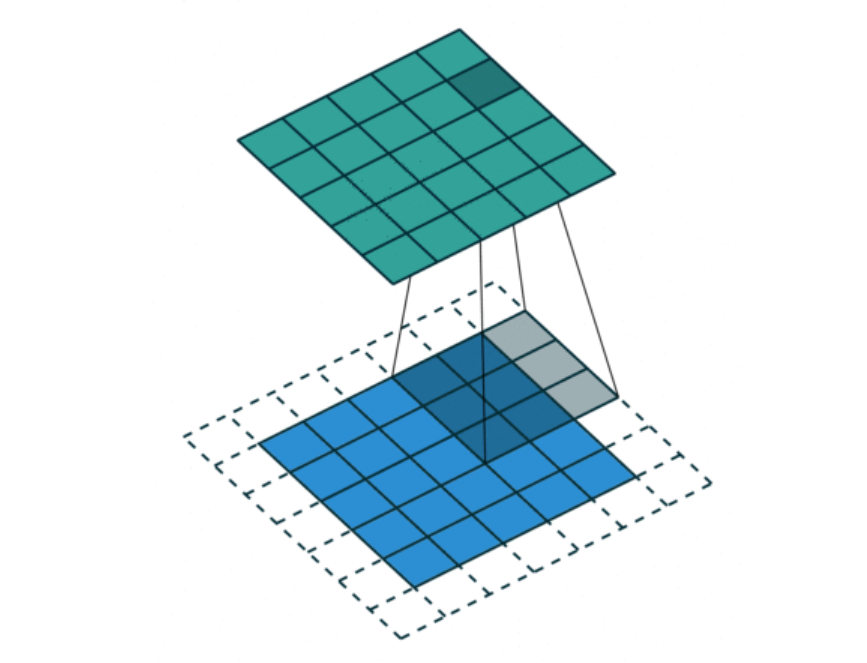
\includegraphics[width = 0.5\textwidth]{conv2d.png}
  \label{fig:conv2d}
  \caption{Convolucion en dos dimensiones con padding.\cite{imConv2d}}
\end{figure}

\par En la figura \ref{fig:conv2d} se observa una imagen de entrada (representada por la matriz de cuadrados azules) con 5 pixeles de ancho por 5 de largo. Adicionalmente, se agrega un pixel de ancho y uno de largo de color blanco. Éstos representan el \textit{padding}.El kernel por otro lado, se representa por los pixeles sombreados (kernel de 3x3).

\par Para el cálculo de la imagen de salida, se utiliza la siguiente ecuación:

\begin{align}
  y[i,j] = \sum_{m}^{M} \sum_{n}^{N} x[i-m, j-n] \cdot h[m,n] \: \: \: \: \forall i \in [0,Height], \: j \in [0,Width]
  \label{eqn:conv2d}
\end{align}

\par En la ecuación \ref{eqn:conv2d}, la imagen de salida (y), se construye con la operación del kernel (h) sobre todos los pixeles de la imagen de entrada (x) y los vecinos correspondientes.

\par En el ejemplo de la figura, se realiza \textit{padding}. Esto consiste en agrandar la imagen de entrada para que la salida sea de la misma dimension. En esta ocación, se realizará padding con ceros, es decir, se rellenará con ceros donde sea necesario.

\subsection{Pirámides}
Como se menciono anteriormente, las pirámides corresponden a representaciones multi-resolución calculadas a partir de imágenes. En éstas, la señal o imagen de entrada es filtrada y submuestreada tantas veces como niveles se quieran.


\par Inicialmente, las pirámides se utilizaron para la detección e identificación de objetos que pueden o no aparecer a distintas escalas. La idea, es crear distintas copias del objeto cambiando el tamaño (o escala) y resolución de estos. En la figura \ref{fig:pyramidPaper} se observan distintas resoluciones del mismo objeto para obtener otras representaciones.

\begin{figure}[H]
  \centering
  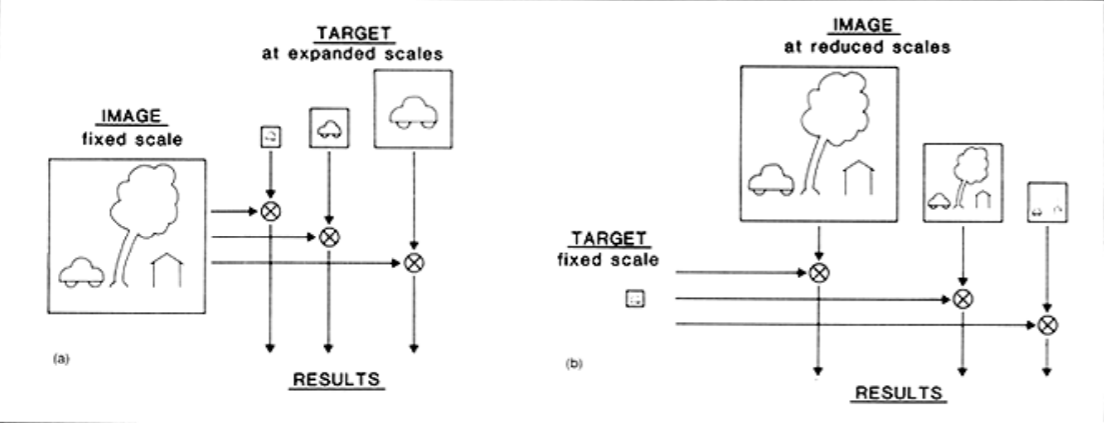
\includegraphics[width = 0.7\textwidth]{pyramid_paper.png}
  \caption{Distintas formas de utilizar las pirámides. En (a), copias del objeto a detectar se escalan. En (b), la imagen se trabaja completa. \cite{paperPyramids}}
  \label{fig:pyramidPaper}
\end{figure}


\subsubsection{Piramide de Gauss}
La pirámide de gauss corresponde a un caso particular de las pirámides en las que el filtro aplicado es uno pasabajo, con semejanzas a un filtro con distribución \textit{gaussiana}. 

\par En estos, se aplica un filtro \textit{gaussiano} a cada imagen y luego se sub-muestrea. El filtro  \textit{gaussiano} también se conoce como \textit{blur} y recibe como parámetro la desviación estándar a partir de la cual se originará el filtro. En la siguiente figura, se observa el efecto de variar la desviación estándar usada para el cálculo del filtro:

\begin{figure}[H]
  \centering
  \begin{subfigure}[t]{0.32\textwidth}
    \centering
    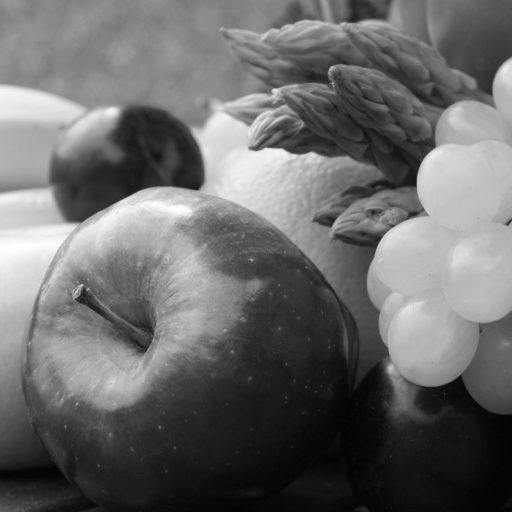
\includegraphics[width = 0.9\textwidth]{frutas.png}
    \caption{Imagen original (en blanco y negro).}
  \end{subfigure}
  ~
  \begin{subfigure}[t]{0.32\textwidth}
      \centering
      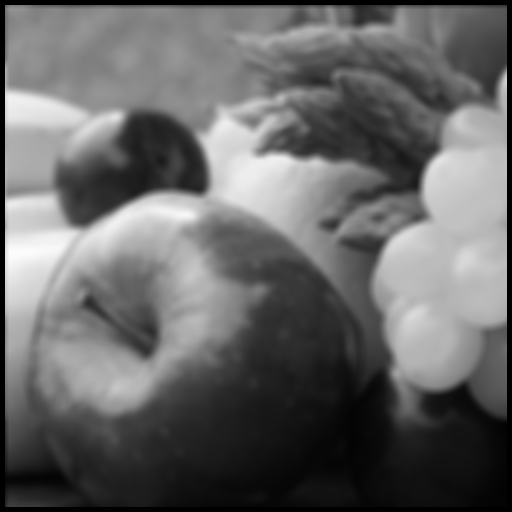
\includegraphics[width = 0.9\textwidth]{frutas_std5.png}
      \caption{Imagen con filtro \textit{blur} aplicado con $\sigma=5$.}
  \end{subfigure}
  ~ 
  \begin{subfigure}[t]{0.32\textwidth}
      \centering
      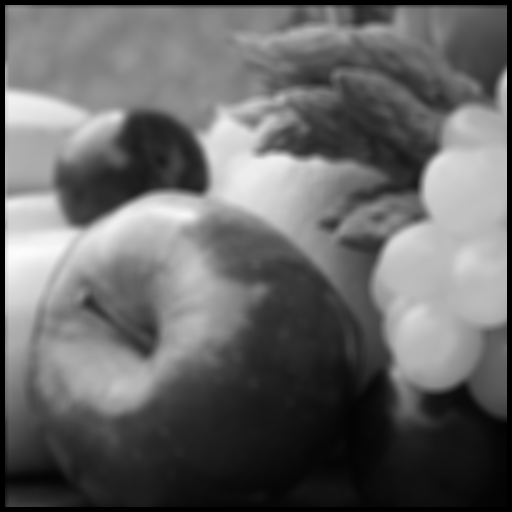
\includegraphics[width = 0.9\textwidth]{frutas_std10.png}
      \caption{Imagen con filtro \textit{blur} aplicado con $\sigma=10$.}
  \end{subfigure}
  \caption{Misma imagen con distintos filtros \textit{blur} aplicados (distinto $\sigma$ mismo tamaño de kernel, 10). }
  \label{fig:frutas}
\end{figure}

\par En la figura se observa el efecto de aumentar $\sigma$. Por otro lado, en los bordes de las figuras \ref{fig:frutas} (a) y (b), se observan los bordes negros que corresponden al \textit{padding} mencionado anteriormente. 


\subsubsection{Piramide de Laplace}
Estas pirámides se construyen con la información perdida en la pirámide de Gauss. Para esto, se resta el nivel actual de la pirámide de Gauss con el siguiente (antes del sub-muestreo). El último nivel de la pirámide de Laplace corresponde al último nivel de la pirámide de gauss.

\bigskip
\par En las figuras \ref{fig:gp3frutas} y \ref{fig:lp3frutas}, se muestran 3 niveles de la piramide de gauss y laplace respectivamente. Éstas fueron generadas a partir de la implementación de la tarea:

\begin{figure}[H]
  \centering
  \begin{subfigure}[t]{0.32\textwidth}
    \centering
    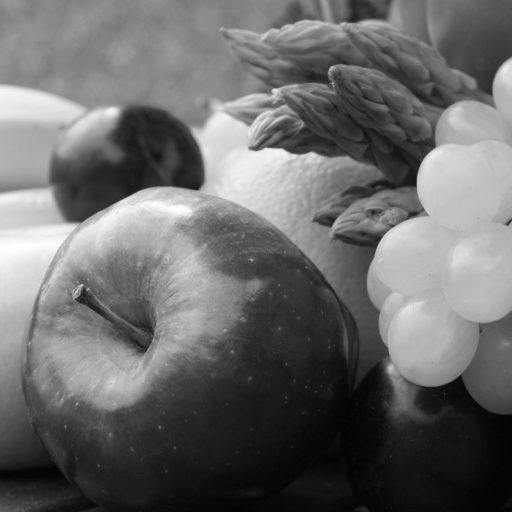
\includegraphics[width = 0.9\textwidth]{piramides/gp1.png}
    \caption{Nivel 1.}
  \end{subfigure}
  ~
  \begin{subfigure}[t]{0.32\textwidth}
      \centering
      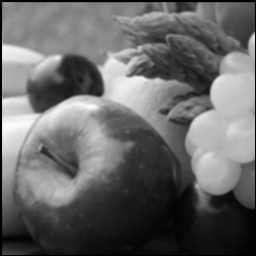
\includegraphics[width = 0.45\textwidth]{piramides/gp2.png}
      \caption{Nivel 2.}
  \end{subfigure}
  ~ 
  \begin{subfigure}[t]{0.32\textwidth}
      \centering
      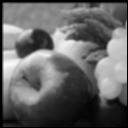
\includegraphics[width = 0.22\textwidth]{piramides/gp3.png}
      \caption{Nivel 3.}
  \end{subfigure}
  \caption{Pirámide de Gauss de 3 niveles.}
  \label{fig:gp3frutas}
\end{figure}

\begin{figure}[H]
  \centering
  \begin{subfigure}[t]{0.32\textwidth}
    \centering
    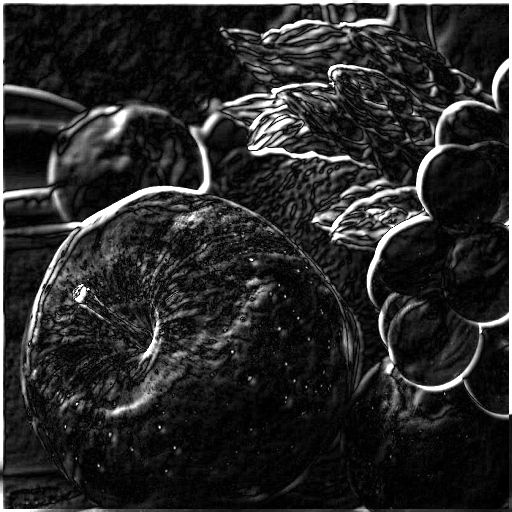
\includegraphics[width = 0.9\textwidth]{piramides/lp1.png}
    \caption{Nivel 1.}
  \end{subfigure}
  ~
  \begin{subfigure}[t]{0.32\textwidth}
      \centering
      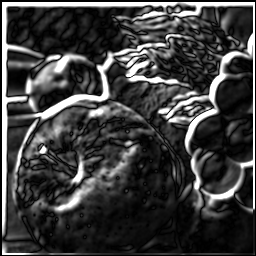
\includegraphics[width = 0.45\textwidth]{piramides/lp2.png}
      \caption{Nivel 2.}
  \end{subfigure}
  ~ 
  \begin{subfigure}[t]{0.32\textwidth}
      \centering
      
\includegraphics[width = 0.22\textwidth]{piramides/lp3.png}
      \caption{Nivel 3.}
  \end{subfigure}
  \caption{Pirámide de Laplace de 3 niveles.}
  \label{fig:lp3frutas}
\end{figure}


\subsection{Reconstrucción de la imagen original}
El proceso de reconstrucción de la imagen a partir de la pirámide de Laplace consiste en, a partir del nivel más profundo de la pirámide repetir lo siguiente:
\begin{enumerate}
  \item Duplicar el tamaño de la imagen.
  \item Sumar la imagen duplicada con el siguiente piso de la pirámide de Laplace. 
\end{enumerate}

\par Para duplicar el tamaño de la imagen, se utiliza interpolación. Es importante destacar que, la imagen reconstruida contiene ciertos artefactos en particular en los bordes. Esto se debe a que al hacer padding (basicamente rellenar con ceros), se pierde información de la imagen original: 


\begin{figure}[H]
  \centering
  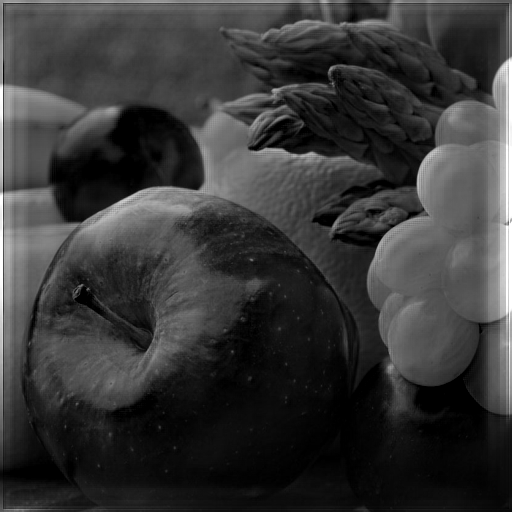
\includegraphics[width = 0.5\textwidth]{frutas_recons.png}  
  \label{fig:frutasRec}
  \caption{Reconstrucción de la imagen de frutas a partir de la pirámide de Laplace de 3 niveles.}
\end{figure}


\bigskip
\bigskip
\bigskip
\bigskip
\bigskip
\bigskip
\par En la siguiente sección, se encuentra la implementación de todo lo descrito.  Por cada ítem, se muestra el código, explicación breve donde sea necesario y una prueba de la función implementada o el resultado que arroja esta. 
 
% \bigskip  
% \par Describir operación de convolución
% \par Describir brevemente cálculo de la pirámide de Gauss
% \par Describir brevemente cálculo de la pirámide de Laplace
% \par Describir brevemente reconstrucción de la imagen original


\newpage
\section{Desarrollo}
\subsection{Pirámide de \textit{Gauss}:}

\subsubsection{Convolución:}
\par A continuación, se presenta el código de la implementación de la convolución en \textit{Cython}:

\begin{lstlisting}[language=Python, label = code:convCode, caption=Implementación de convolución en Cython.]
  cpdef float[:, :] convolution_cython(float [:, :] input, float [:, :] mask):
  cdef int a, b, r, c, rows, cols, row_init, col_init, i, j,
  cdef float sum
  # Imagen de salida
  cdef np.ndarray output=np.zeros([input.shape[0], input.shape[1]], dtype = np.float32)

  # Posicion a partir de la cual se puede realizar convolucion: 
  # Ejemplo 1: Para un kernel de 3x3, es (1,1).
  # Ejemplo 2: Para un kernel de "a" x "b" es ("r"//2, "c"//2)
  a = mask.shape[0]
  b = mask.shape[1]

  row_init = a // 2
  col_init = b // 2

  # tamano de la imagen
  rows = input.shape[0]
  cols = input.shape[1]

  sum = 0

  # Recorremos la imagen input:
  for r in range(row_init, rows - row_init):
    for c in range(col_init, cols - col_init):
      # Se recorre la mascara o kernel:
      for i in range(a):
        for j in range(b):
          sum += mask[i,j] * input[r-i,c-j]
      # Guardamos el resultado de la suma correspondiente en el arreglo output:
      output[r, c] = sum
      sum = 0
  return output
\end{lstlisting}

\par La implementación en \ref{code:convCode}, corresponde a la convolución en dos dimensiones con padding. En el código, la sección más importante corresponde a los 4 ciclos de iteraciones anidados. Estos son los que recorren en primer lugar la imagen (\texttt{for r in rows} y luego \texttt{for c in columns}) y luego el \textit{kernel} guardando en la variable \texttt{sum} el resultado de operar para cada pixel \texttt{(r,c)} de la imagen, el resultado de la operación convolución. 

\par Es importante destacar que esta función se implementó en \textit{Cython} para intentar ganar eficiencia. Para verificar si era más rápida o no que una implementación de librerías, se comparó con la función \texttt{signal.convolve2d} de la librería \texttt{Scipy}. Para esto, se utilizó la herramienta de perfilamiento (\texttt{\%timeit}) de Python. Esta ejecuta cierta cantidad de veces la función pedida (100 veces en este caso) y entrega el mejor resultado obtenido. Adicionalmente, prueba (si hay disponible) en los distintos \textit{cores} del computador:


\begin{table}[H]
  \centering
  \begin{tabular}{|c|c|c|}
  \hline
                          & \textit{\textbf{Cython}} & \textit{\textbf{Scipy}} \\ \hline
  \textbf{Timpo {[}ms{]}} & $18.2$                     & $6.11$                    \\ \hline
  \end{tabular}
  \label{table:profile}
  \caption{Tiempos de ejecución de operación convolución.}
\end{table}

\par Se observa en la tabla \ref{table:profile} que la función del módulo \textit{scipy} es tres veces mas rápida. De todas formas, se continuará utilizando la función implementada en \textit{cython}, siguiendo las instrucciones del enunciado.

\par A continuación, se muestra la imagen de salida al ejecutar lo siguiente:
\begin{lstlisting}[language=Python, label = code:convCodeejec, caption=Implementación de convolución en Cython.]
  Holoquetal = 
\end{lstlisting}

\bigskip
- Describir implementación de convolución, incluyendo código
- Describir implementación de cálculo de máscaras, incluyendo código
- Describir implementación de suavizado de imágenes, incluyendo código
- Describir implementación de submuestreo, incluyendo código
- Describir implementación de pirámide de Gauss, incluyendo código
- Describir implementación: graficar pirámide de Gauss, incluyendo código
- Prueba del sistema de cálculo de pirámide de Gauss sobre 4 imágenes entregadas, incluir las
imágenes de las pirámides resultantes en el informe
- Análisis del desempeño del cálculo de la pirámide de Gauss, analizando las imágenes resultantes


\subsection{Pirámide de \textit{Laplace}:}
- Describir implementación de resta de imágenes, incluyendo código
- Describir implementación de pirámide de Laplace, incluyendo código
- Describir implementación de valor absoluto y escalamiento, incluyendo código
- Describir implementación: graficar pirámide de Laplace, incluyendo código
- Prueba del sistema de cálculo de pirámide de Laplace sobre 4 imágenes entregadas, incluir las
imágenes de las pirámides resultantes en el informe
- Análisis del desempeño del cálculo de la pirámide de Laplace, analizando las imágenes resultantes


\subsection{Reconstrucción imagen:}
- Describir implementación de suma de imágenes, incluyendo código
- Describir implementación de duplicación de tamaño de imágenes con interpolación, incluyendo
código
- Describir implementación de reconstrucción de imagen original, incluyendo código
- Prueba del sistema de reconstrucción de la imagen original usando las pirámides de las cuatro
imágenes entregadas, incluir las imágenes reconstruidas en el informe
- Análisis del resultado de la reconstrucción respecto a las imágenes originales


\section{Conclusión}


\newpage
\begin{thebibliography}{X}
    \bibitem{WikiConv} Wikipedia: Convolution. \\
    \url{https://en.wikipedia.org/wiki/Convolution#Visual_explanation} 

    \bibitem{imConv2d} Towards Data Science: Intuitively Understanding Convolutions for Deep Learning. By Irhum Shafkat. \\
    \url{https://towardsdatascience.com/intuitively-understanding-convolutions-for-deep-learning-1f6f42faee1} 

    \bibitem{paperPyramids} Pyramid methods in image processing. E. H. Adelson, C. H. Anderson,  J. R. Bergen,  P. J. Burt,  J. M. Ogden. $[1984]$
    \url{http://persci.mit.edu/pub_pdfs/RCA84.pdf}

\end{thebibliography}

\section{Anexos}
\end{document}